\documentclass[12pt, onecolumn]{article}

\usepackage[margin=1in]{geometry}
\usepackage{amsmath}
\usepackage{amssymb}
\usepackage{graphicx}
\usepackage{cite}
\usepackage{setspace}
\usepackage{listings}
\usepackage{xcolor}
\usepackage{float}
\usepackage{booktabs}
\usepackage{hyperref}

\singlespacing 

\lstset{
    language=Python,
    basicstyle=\ttfamily\footnotesize, % Base font style and size
    keywordstyle=\color{blue!60!black},
    commentstyle=\color{green!50!black},
    stringstyle=\color{teal!60!black},
    numbers=left,                      % line numbers on the left
    numberstyle=\tiny\color{gray},
    stepnumber=1,                      % line numbers every 1 line
    breaklines=true,                   % Wrap long lines
    breakatwhitespace=false,           % Line break anywhere if needed
    columns=flexible,                  % Better spacing between characters
    frame=single,                      % Add a frame around the code
    tabsize=4,                         % Set tab size to 4 spaces
    showstringspaces=false,
    inputencoding=utf8,
    extendedchars=true
}

\begin{document}

% ----------------------------------------------------------------------
% TITLE PAGE
% ----------------------------------------------------------------------

\begin{titlepage}
    \centering
    \vspace*{50pt}
    {\Large \textbf{The Transported Probability Density Function (PDF) Method and its Relation to the Black-Scholes-Merton Equation} \par}
    \vspace{25pt}
    {\Large Christian DiPietrantonio \par}
    \vfill
    {\large ME 5311: Computational Methods to Viscous Flows \par}
    {\large University of Connecticut \par}
    {\large \today \par}
    \vspace{50pt}
\end{titlepage}

% ----------------------------------------------------------------------
% TITLE PAGE
% ----------------------------------------------------------------------
\pagenumbering{roman}
\tableofcontents
\newpage
\pagenumbering{arabic}

% ----------------------------------------------------------------------
% SECTION 01: INTRODUCTION
% ----------------------------------------------------------------------
\section{Introduction}

This paper explores the mathematical connection between the Black-Scholes-Merton (BSM) equation for pricing financial derivatives and the transported probability density function (PDF) method employed in computational fluid dynamics (CFD). The central argument is that these two equations, from completely different fields, are derived from stochastic differential equations (SDEs) of the same dift plus diffusion form, and can be solved using the same classes of numerical methods. The BSM equation is derived from the geometric brownian motion SDE, while the transported PDF equation is derived from the generalized Langevin SDE for the velocity of a fluid particle in turbulence. Even though the two equations were developed in separate disciplines, these two equations share a mathematical connection through stochastic calculus.

The paper begins by establishing the financial definitions and background necessary to the understanding of the further sections. Following this, the BSM equatin is derived following the approach outlined by Hull~\cite{Hull2022} and Merton~\cite{Merton1973}. The transporded PDF method is then introduced following the work of Pope~\cite{Pope2000}, and the connection between it and the BSM equation is illustrated through comparison of the underlyinbg SDEs and variable mapping. The paper then outlines the solution methods for the BSM and the transported PDF equation, which include grid-based {Eulerian} and particle-based {Lagrangian} approaches. To demonstrate these solution methods, a Python program was developed that implements three different solution methods for pricing a European call option. The first solution method is simply the analytical solution to the BSM equation. Following this, the solver implements an implicit finite difference scheme (Eulerian approach), and a Monte Carlo simulation (Lagrangian approach). The results are compared to one another, and also used to visualize the transport of the probability density function of the stock price. The latter of which can be directly related to the transported PDF of a the velocity of a fluid particle as obtained by the transported PDF method. The benefits and pitfalls of the different solution approaches are also explored. Finally, the paper concludes by discussing the real-world applications of this cross-disciplinary connection, and how advancements in either quantitative finance or computational fluid dynamics have potential to be utilized by the other.

To begin the comparison of the equations and methods, a foundational understanding of the Black-Scholes-Merton equation is necessary.~\cite{Hull2022}

% ----------------------------------------------------------------------
% SECTION 02: FINANCIAL DERIVATIVES AND THE BSM EQUATION
% ----------------------------------------------------------------------
\section{Financial Derivatives and the Black-Scholes-Merton Equation}

\subsection{Financial Derivatives and Options}

In order to understand the Black-Scholes-Merton equation, a foundational understanding of financial derivatives, specifically options, is required. According to Hull, a derivative is a ``financial instrument whose value depends on (or derives from) the values of other, more basic, underlying variables''~\cite{Hull2022}. A stock option, for example, is a derivatve whose value is dependant on the price of a stock. However, different derivatives can be dependant on almost any variable, even the weather. For this paper, the primary derivatives of interest are options, which are securities that give ``the right to buy or sell an asset, subject to certain conditions, within a specified period of time''~\cite{BlackScholes1973}.

The two major types of options are call and put options. A call option gives the holder the right, but not the obligation, to buy the underlying asset by a certain data for a certain price. A put option gives the holder the right, but not the obligation, to sell the underlying asset by a certain data for a certain price~\cite{Hull2022}. Options can also be further classified by when they can be excercised. American options can be excercised at any time up to the expiration date as specified in the contract, while European options can only be excercised on the expiration date itself~\cite{BlackScholes1973}. The price at which the asset may be bought or sold is refered to as the strike price, $K$, and the expiration date can an also be refrered to as the maturity date, $T$.

For the remainder of this paper, the focus will be on European call options. The value of a European call option at expiry can be determined by the following payoff function:
\begin{equation}
    V = \max(S_T - K)
\end{equation}
Where $S_T$ is the stock price at expiry. From this payoff function one can observe that, if the stock price exceeds the strike price at expiry, the holder profits. However, if the stock price at expiry is below the strike price, the option expires worthless, as the holder is not obligated to execute the option. In this latter scenario, the holder only loses what they paid for the option. The Black-Scholes-Merton equation aims to determine a price for the contract, before its value is known at expiry.

\subsection{The Black-Scholes-Merton Equation}

In deriving their valuation formula, Black and Scholes~\cite{BlackScholes1973} assume an idealized, frictionless market with continuous trading, no transaction costs, constant interest rates, no dividends, unrestricted short selling, and the ability to borrow or lend at the risk-free rate. The option is also assumed to be a European call option. Furthermore, an arbitrage-free market is also assumed, which means that no trading strategy can generate riskless profits. More explicitly, an arbitrage opportunity can be formally defined as “a (self-financing) trading strategy” that starts with zero value and terminates with a positive value. Therefore, a market is arbitrage-free if there are no such arbitrage opportunities~\cite{BaxterRennie1996}.

The assumptions outlined above lead to the derivation of the following second-order linear parabolic Partial Differential Equation (PDE) for the price $V(S,t)$ of a European call option. The same equation was independently derived by Robert C. Merton~\cite{Merton1973} through the use of stochastic calculus, and therefore is commonly referred to as the Black-Scholes-Merton PDE:
\begin{equation}
    \frac{\partial V}{\partial t} + \frac{1}{2} \sigma^2 S^2 \frac{\partial^2 V}{\partial S^2} + rS \frac{\partial V}{\partial S} - rV = 0
    \label{eq:bsm}
\end{equation}

\noindent Where $S$ is the underlying stock price, $t$ is time, $r$ is the risk-free interest rate, and $\sigma$ is the volatility of the stock, a measure of how much the stock price fluctuates, or in other words a “measure of our uncertainty about the returns provided by the stock”~\cite{Hull2022}. This equation was obtained by forming a hedged portfolio that eliminates risk and requiring that its returns equal the risk-free rate in an arbitrage-free market.

It should also be noted that the structure of Equation~\ref{eq:bsm} can be recognized as having the same form of the general transport equation given the context of this course. Where $\frac{\partial V}{\partial t}$ is the temporal term, $\frac{1}{2} \sigma^2 S^2 \frac{\partial^2 V}{\partial S^2}$ is a diffusion term, $rS \frac{\partial V}{\partial S}$ is an advection term, and $rV$ is a source (in this case, decay) term. This course has dedicated ample time to discritizing and computatonally solving equations of this exact form.

% ----------------------------------------------------------------------
% SECTION 03: DERIVATION OF THE BSM EQUATION
% ----------------------------------------------------------------------
\section{Derivation of the Black-Scholes-Merton Equation}

The use of Stochastic Calculus in the derivation of Equation~\ref{eq:bsm} is crucial to the argument of this paper. Therefore, this section will walk through such derivation as done so by Hull~\cite{Hull2022} and Merton~\cite{Merton1973}.

\subsection{Stochastic Calculus and It\^{o}'s Lemma}

GO TO SHREVE FOR DEFINITION OF STOCHASTIC CALCULUS

Before completing the derivation, it is important to highlight a few concepts from Stochastic Calculus that are used in the derivation. First, it should be noted that Stochastic Calculus is a branch of mathematics built specifically to handle the derivatives and integrals of stochastic processes, which are by definition, ``an equation describing the probabilistic behavior of a stochastic variable''~\cite{Hull2022}. Furthermore, a stochastic variable can be defined as a variable ``whose future is uncertain'', or in other words, random. The first process to consider is the generalzied Wiener process:
\begin{equation}
    dx = adt + bdz
\end{equation}
Where $dz = \epsilon \sqrt{\Delta t}$ is refered to as a Wiener process, and $\epsilon$ has a standard normal distribution. Further, an It\^{o} process is a generalized Wiener process where the parameters $a$ and $b$ are functions of the underlying variable and time, and can be expressed as:
\begin{equation}
    dx = a(x, t)dt + b(x, t)dz
    \label{eq:ito_process}
\end{equation}
In standard calculus, the chain rule can be used to find the derivative or differential of a multivariable function. However, in Stochastic Calculus, one must use It\^{o}'s Lemma to compute the stochastic differential of a function that depends on a stochastic process. Doing so accounts for the fact that second-order terms can not be ignored in the formulation of the differential. This is because the diffusion term in a stochastic process (at least the ones within the scope of this paper) depends on a Wiener Process $dz \sim \sqrt{\Delta t}$, and when squared, this term is on the order of $dt$.
It\^{o}'s lemma shows that for a function $G(x, t)$, where $x$ is a stochastic variable following an It\^{o} process, the differential of $G$ can be expressed as
\begin{equation}
    dG = \frac{\partial G}{\partial x} dx + \frac{\partial G}{\partial t} dt + \frac{1}{2} \frac{\partial^2 G}{\partial x^2} b^2 dt
    \label{eq:ito_lemma}
\end{equation}
Again, the key difference from ordinary calculus is the presence of the second-order term $\frac{\partial^2 G}{\partial x^2} b^2$~\cite{Hull2022}.

\subsection{The Stock Price Model: Geometric Brownian Motion}

Returning to the topics of this paper, the price of a stock $S$ is modeled as a stochastic process using the following stochastic differential equation:
\begin{equation}
    dS = rS\, dt + \sigma S\, dW
    \label{eq:gbm}
\end{equation}
where $r$ is the stocks expected rate of return (in this case, the risk-free rate), $\sigma$ is the volatility of the stock price, and $dW$ is a Wiener process (analagous to $dz$)~\cite{Hull2022, Shreve2004}. This model is commonly refered to as geometric Brownian motion. The first term, $rS\, dt$, represents the deterministic drift of the stock's price, and the second term, $\sigma S\, dW$ represents random variance.

\subsection{Applying It\^{o}'s Lemma to the Option Value}

Suppose $V(S, t)$ is the value of a European call option dependant on the price of stock $S$. Given that the price of $S$ is modled using the It\^{o} process above, It\^{o}'s lemma (Equation~\ref{eq:ito_lemma}) can be applied, and the result can be rearranged using Equation~\ref{eq:gbm} to obtain:
\begin{equation}
    dV = \left(rS\frac{\partial V}{\partial S} + \frac{\partial V}{\partial t} + \frac{1}{2}\sigma^2 S^2 \frac{\partial^2 V}{\partial S^2}\right)dt + \frac{\partial V}{\partial S}\sigma S\,dW
    \label{eq:dV}
\end{equation}

Since the Wiener processes in Equatiion~\ref{eq:gbm} and Equation~\ref{eq:dV} are the same, a portfolion consisting of positions in both the option and the stock can be created such that the Wiener process is eliminated~\cite{Hull2022}.

\subsection{Constructing the Hedged Portfolio}

This portfolio as created by Hull, consists of a short position (selling) in one derivative and a long posiiton (buying) in $\frac{\partial V}{\partial S}$ shares of the underlying stock.
\begin{equation}
    \Pi = -V + \frac{\partial V}{\partial S} S
    \label{eq:hedged_portfolio}
\end{equation}

The change in this portfolio over a smal time interval, $dt$, can be expressed as:
\begin{equation}
    d \Pi = - dV + \frac{\partial V}{\partial S}\, dS
\end{equation}

The expressions above for $dV$ (Equation~\ref{eq:dV}) and $dS$ (Equation~\ref{eq:gbm}) can be substituted into the equation above to obtain:
\begin{equation}
    d\Pi = \left(- \frac{\partial V}{\partial t} - \frac{1}{2}\sigma^2 S^2 \frac{\partial^2 V}{\partial S^2}\right)dt
    \label{eq:portfolio_change}
\end{equation}

As expected, the Wiener processes cancel, eliminating randomness fromt the expression.

\subsection{No Arbitrage Condition}

Hull states that because this expression is now free of the randomness induced by the Wiener process, it must be riskless. Therefore, due to the no arbitrage assumption, the portfolio must grow with the risk free rate:
\begin{equation}
    d Pi = r\, \Pi\, d t
\end{equation}

Subsituting Equation~\ref{eq:hedged_portfolio} and Equation~\ref{eq:portfolio_change} then yields:
\begin{equation}
    \left(\frac{\partial V}{\partial t} + \frac{1}{2}\sigma^2 S^2 \frac{\partial^2 V}{\partial S^2}\right)dt = r\left(V - \frac{\partial V}{\partial S}S\right)dt
\end{equation}

Then, dividing both sides by $dt$ and rearranging yields the Black-Scholes Merton PDE exactly as seen in Equation~\ref{eq:bsm}
\begin{equation}
    \frac{\partial V}{\partial t} + \frac{1}{2}\sigma^2 S^2 \frac{\partial^2 V}{\partial S^2} + rS\frac{\partial V}{\partial S} - rV = 0
\end{equation}

% ----------------------------------------------------------------------
% SECTION 04: THE TRANSPORTED PDF METHOD
% ----------------------------------------------------------------------
\section{The Transported PDF Method}

\subsection{Statistical Description of Turbulent Flows}

In \textit{Turbulent Flows}, Stephen B. Pope remarks that “in a turbulent flow, the velocity field $U(x,t)$ is random”~\cite{Pope2000}. This means that if one were to repeat the same experiment multiple times under the same set of conditions, a given event may, but need not occur, making the event inherently unpredictable. Although a random variable, such as velocity, can not be predicted, the probability of events (e.g., the velocity is less than 10 m/s) can be used to create a Probability Density Function (PDF) that characterizes the random variable. Formally, the probability of any event can be determined by the Cumulative Distribution Function, and the PDF is defined to be the derivative of the CDF. Therefore, according to Pope, a random variable such as the velocity of a turbulent fluid, is completely characterized by its PDF, which can be thought of as the probability per unit distance in the sample space ~\cite{Pope2000}.


\subsection{Eulerian PDF Transport Equation}

The evolution of this Eulerian PDF of velocity in space and time can be represented by a transport equation derived by Pope from the Navier-Stokes equations. The result is the following Eulerian PDF transport equation:
\begin{equation}
    \frac{\partial f}{\partial t} + V_i \frac{\partial f}{\partial x_i} = - \frac{\partial}{\partial V_i} \left[f \left \langle \frac{DU_i}{Dt} \middle| \mathbf{V} \right \rangle \right]\
    \label{eq:eulerian_pdf}
\end{equation}

\noindent Where $f(\mathbf{V}; \mathbf{x}, t)$ is the Eulerian PDF of velocity.

\subsection{The Generalized Langevin Model}

To model the evolution of fluid particle velocities, Pope introduced the generalized Langevin model for a diffusion process. The Langevin equation was originally proposed in 1908 as a stochastic model for the velocity of a microscopic particle undergoing Brownian motion. Pope states that the equation provides a good model for the velocity of a fluid particle in turbulence~\cite{Pope2000}. The generalized Langevin model used to expresses the velocity of a fluid particle is expressed below:
\begin{equation}
    d\mathbf{U^*}(t) = \mathbf{a}(\mathbf{U^*}(t), \mathbf{X^*}(t), t)\,dt + b(\mathbf{X^*}(t), t)\,d\mathbf{W}
    \label{eq:langevin}
\end{equation}
where $\mathbf{a}(\mathbf{U^*}, \mathbf{X^*}, t)$ is the drift coefficient, $b(\mathbf{X^*}, t)$ is the diffusion coefficient, and $d\mathbf{W}$ is a vector-valued Wiener process~\cite{Pope2000}. The drift coefficient effectively describes the direction and speed of the system if no randomness were present, and the diffusion coefficient determines the intensity of the random fluctuations induced by the vector-valued Wiener process~\cite{Pope2000}. According to Pope, the Langevin equation is the simplest stochastic Lagrangian model for a turbulent fluid particle. It should also be noted that The stochastic process $U^*(t)$ is refered to in the text as the Ornstein-Uhlenbeck (OU) process, and although its PDF is already known to evolve by the Fokker-Planck equation~\cite{Pope2000}, Pope still highlights this transition.

\subsection{Derivation of the PDF Transport Equation}

From the Langevin SDE (Equation~\ref{eq:langevin}), It\^{o} calculus can be used to derive the Fokker-Planck equation, which is also known as the forward Kolmogorov equation, and describes the transport of the joint Lagrangian PDF of the particle velocity and position, $ f^{*}_L(\mathbf{V}, \mathbf{x}; t)$. The Fokker-Planck equation can then be divided by the marginal position PDF, $f^{*}_X (\mathbf{x}, t)$ to obtain an expression for the evolution of the conditional PDF of the particle velocity, $f^*\left(\mathbf{V} \middle| \mathbf{x}, t\right)$~\cite{Pope2000}.
\begin{equation}
    \frac{\partial f^*}{\partial t} + V_i \frac{\partial f^*}{\partial x_i} = - \frac{\partial}{\partial V_i} \left[f^* a_i(\mathbf{V}, \mathbf{x}, t)\right] + \frac{1}{2} b{\left(\mathbf{x}, t\right)}^2 \frac{\partial^2 f^*}{\partial V_i \partial V_i}
    \label{eq:lagrangian_pdf}
\end{equation}
Pope notes that the conditional PDF, $f^*$ is the corresponding representation of the Eulerian PDF of velocity, $f$, for a particle system. Therefore, Equation~\ref{eq:lagrangian_pdf} can be thought of as the Lagrangian equvalent of the Eulerian PDF transport equation, Equation~\ref{eq:eulerian_pdf}. As a result, Equation~\ref{eq:lagrangian_pdf} is commonly refered to as the Lagrangian PDF transport equation, and again, it describes the transport of the conditional PDF of the particle velocity~\cite{Pope2000}.

% ----------------------------------------------------------------------
% SECTION 05: THE CONNECTION
% ----------------------------------------------------------------------
\section{The Connection Between the BSM Equation and the Transported PDF Method}

\subsection{Structural Equivalence of the SDEs}

Both the Black-Scholes-Merton and Lagrangian PDF Transport equations are both derived from stochastic differential equations of the same drift plus diffusion form. Comparing the geometric Brownian motion SDE from which the BSM equation is derived (Equation~\ref{eq:gbm}):
\begin{equation*}
    dS = rS\,dt + \sigma S\,dW
\end{equation*}
with the generalized Langevin SDE (Equation~\ref{eq:langevin}) from which the Lagrangian PDF Transport equation is derived:
\begin{equation*}
    d\mathbf{U^*}(t) = \mathbf{a}(\mathbf{U^*}, \mathbf{X^*}, t)\,dt + b(\mathbf{X^*}, t)\,d\mathbf{W}
\end{equation*}
reveals that both equations have the same mathematical structure: deterministic drift term multiiplied by $dt$, plus a diffusion term (random fluctuations) driven by a Wiener process, $dW$. Furthermore, both equations can be derived using the same mathematical tools, Stochastic Calculus and It\^{o}'s lemma.


\subsection{Variable Mapping}

In short, the structural equivalece between the two mathematical frameworks can be summarized through the direct variable mapping:
\begin{table}[H]
    \centering
    \caption{Variable mapping between Black-Scholes-Merton and PDF Transport frameworks}  
    \begin{tabular}{ll}
        \toprule
        \textbf{Quantitative Finance (GBM / BSM)} & \textbf{CFD (Langevin / PDF Transport)} \\
        \midrule
        Stock price, $S$ & Particle velocity, $\mathbf{U^*}$ \\
        Risk-free rate, $r$ & Drift Coefficient, $\mathbf{a}$ \\
        Volatility, $\sigma$ & Diffusion coefficient, $b$ \\
        Wiener process, $dW$ & Vector-valued Wiener process, $d\mathbf{W}$ \\
        Monte Carlo simulation & Langrangian particle method \\
        \bottomrule
    \end{tabular}
    \label{tab:mapping}
\end{table}
However, a few key distinctions should be made. The most prominent is that the BSM equation computes the conditional expectation of a future payoff given the current state, then discounts it back to give the current option price. Wheras, the Lagrangian Transported PDF equation describes how the PDF of velocity evolves over time. In other words, for BSM, the PDF of the stock price is used at expiry (or any future time) to find the expected payoff at that time, then the result is discount it back to its value at a past date. Another different to highlight is that the drift and diffusion coefficients ($r$ and $\sigma$) are constant for the Brownian Motion SDE, while the coefficients in the Langevin SDE ($\mathbf{a}$ and $b$) depend on the particle's velocity and position at a given time. This difference has a significant impact on the availale solution methods and validation techniques, which is discussed in Section~\ref{sec:solution_methods}. Finally, it should be mentioned that the stochastic differential equation for the velocity of a particle uses a vector-valued Wiener process, because the stochastic perturbations act in multiple spatial directions (typically three-dimensional space). Nevertheless, through observing the variable mapping above, a significant connection between not just the two frameworks, but their solution methods as well can be observed.

% ----------------------------------------------------------------------
% SECTION 06: SOLUTION METHODS
% ----------------------------------------------------------------------
\section{Solution Methods}
\label{sec:solution_methods}

Both the Black-Scholes-Merton and Lagrangian Transported PDF equations can be solved using Eulerian (grid-based) and Lagrangian (particle-based) methods.

\subsection{Eulerian Methods}

TBD

\subsection{Lagrangian Methods}

TBD

\subsection{Constant vs. Variable Coefficients}

TBD

% ----------------------------------------------------------------------
% SECTION 07: COMPUTATIONAL EXPERIMENTS AND RESULTS
% ----------------------------------------------------------------------

\section{Computational Experiments and Results}

MAIN PLOT ON OWN FIG \\
MC PATHS \& PDF TRANSPORT (SIDE BY SIDE) \\
FRONT \& TOP VIEWS OF PDF TRANSPORT (SIDE BY SIDE) \\
MC ERROR ON OWN FIG

\subsection{Problem Description}

TBD

\subsection{Analytical Solution}

TBD

\subsection{Finite Difference Solver (Eulerian)}

TBD

\subsection{Monte Carlo Solver (Lagrangian)}

TBD

\subsection{Results: Option Pricing}

\begin{figure}[H]
    \centering
    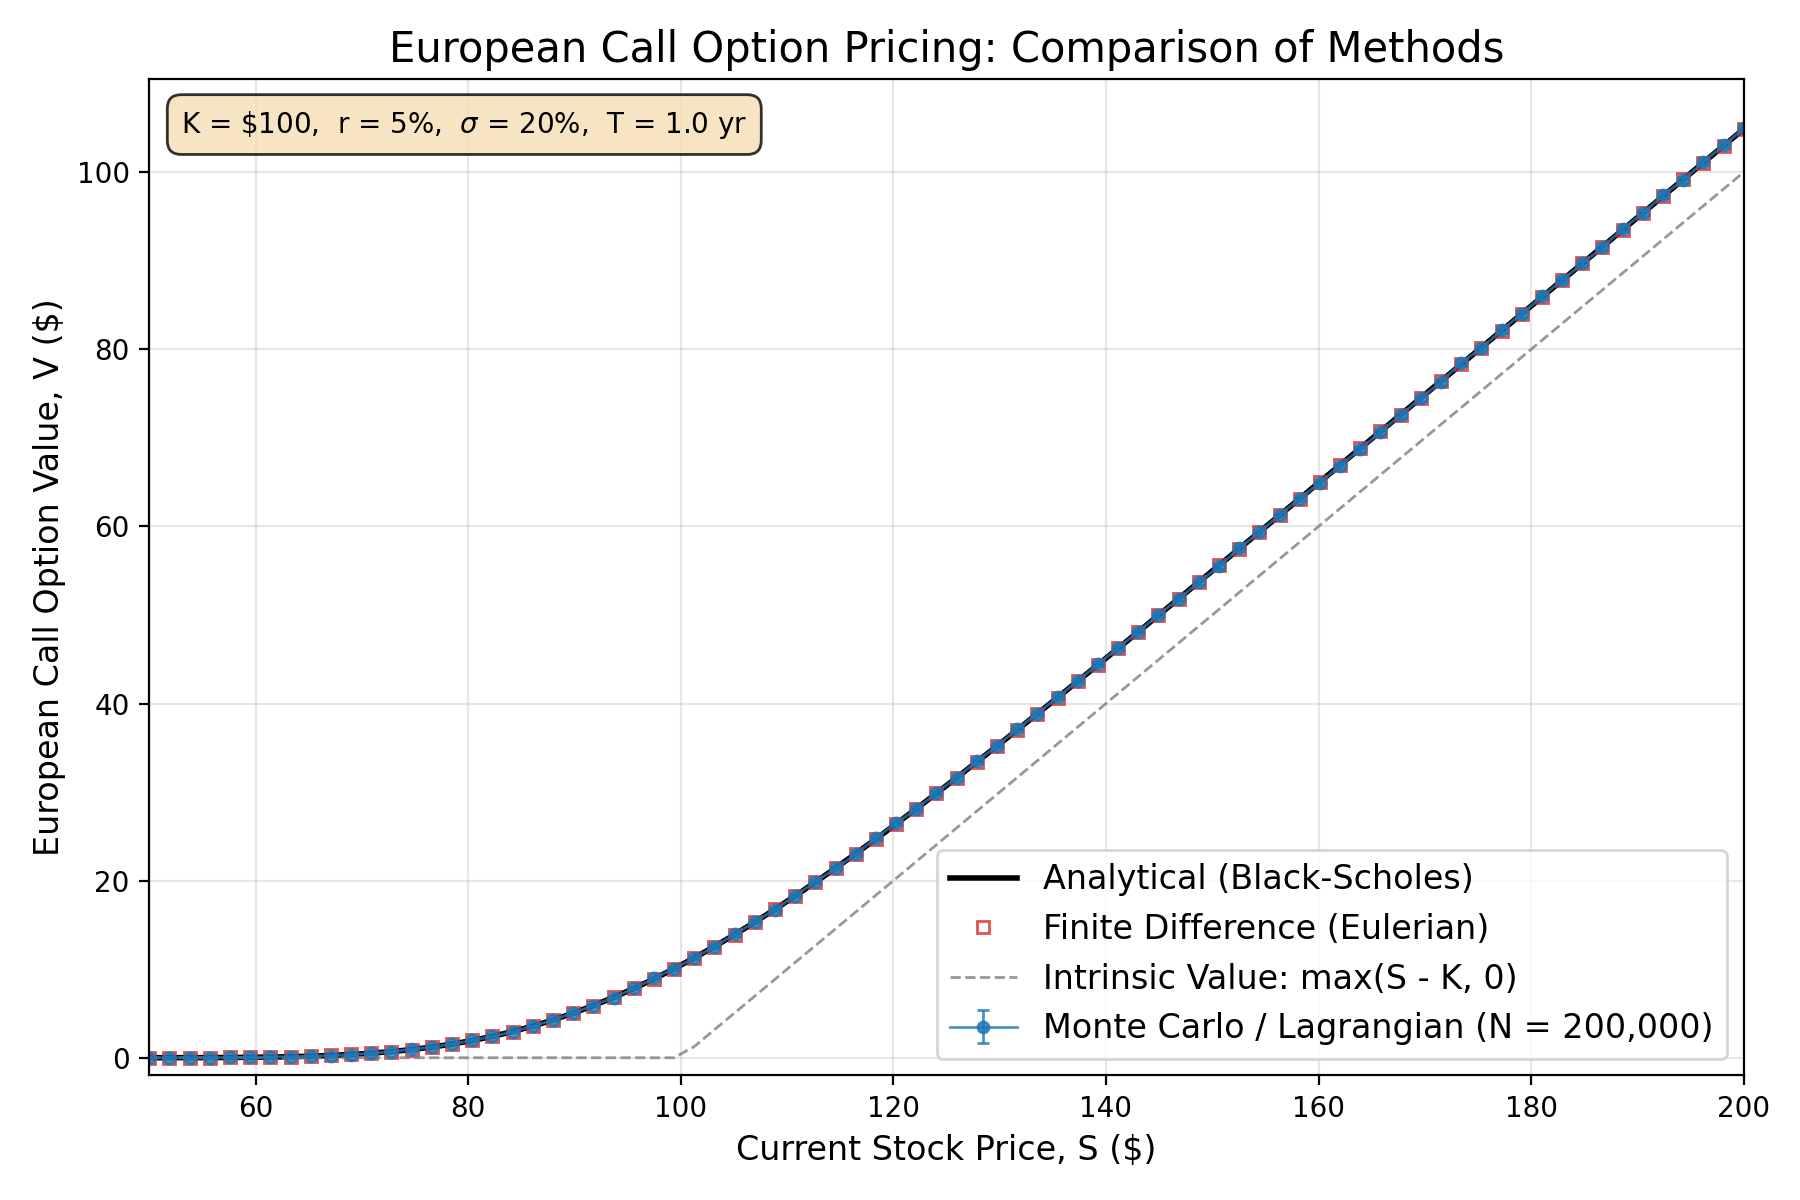
\includegraphics[width=0.85\textwidth]{../BSM_Solver/figures/figure01_option_value_curve.png}
    \caption{European call option value vs.\ stock price: comparison of analytical, eulerian, and lagrangian methods}
    \label{fig:option_value}
\end{figure}

\subsection{Results: Monte Carlo Visualization and PDF Transport}

\begin{figure}[H]
    \centering
    \begin{minipage}[t]{0.45\textwidth}
        \vspace{0pt}
        \centering
        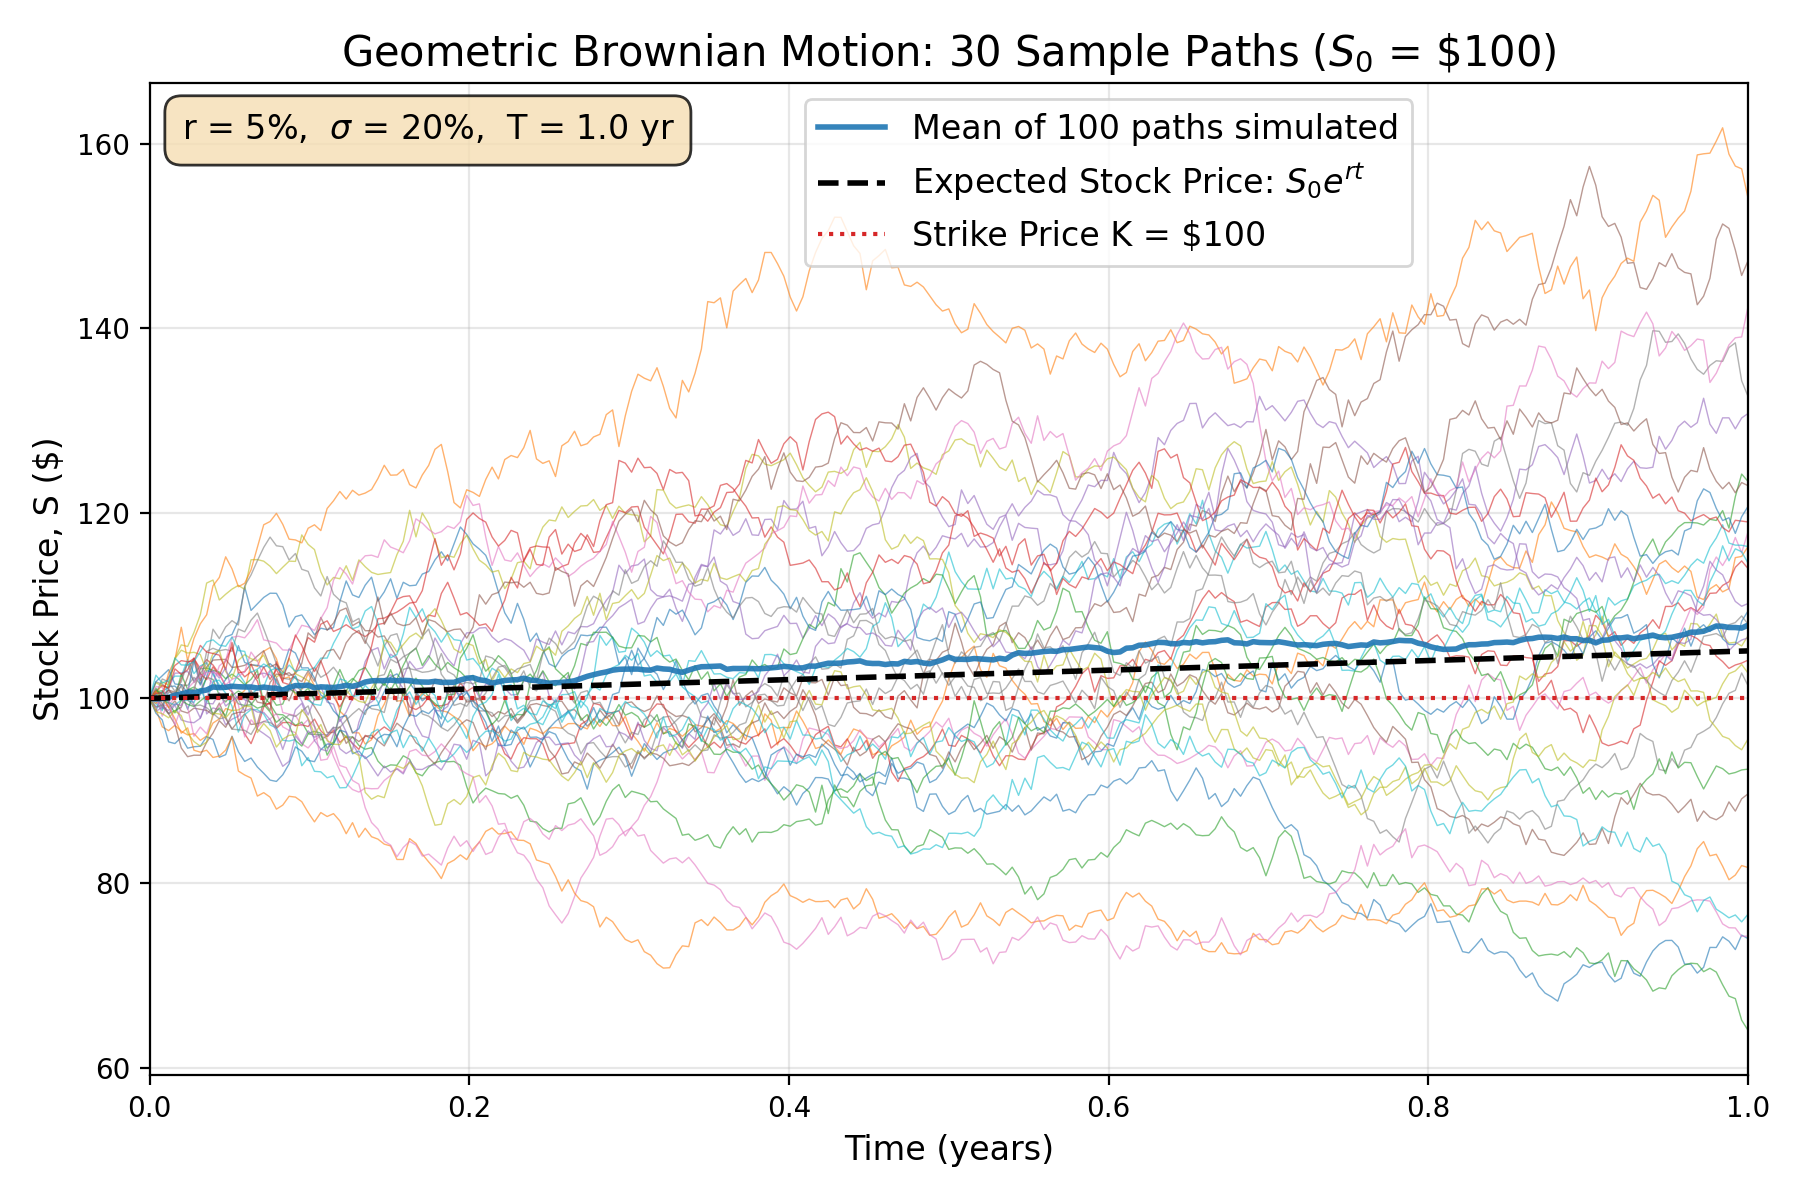
\includegraphics[width=\textwidth]{../BSM_Solver/figures/figure02_GMB_sample_paths.png}
        \caption{Geometric Brownian Motion: 30 sample paths with mean and expected return.}
        \label{fig:loglaw}
    \end{minipage}
    \hspace{8pt}
    \begin{minipage}[t]{0.45\textwidth}
        \vspace{0pt}
        \centering
        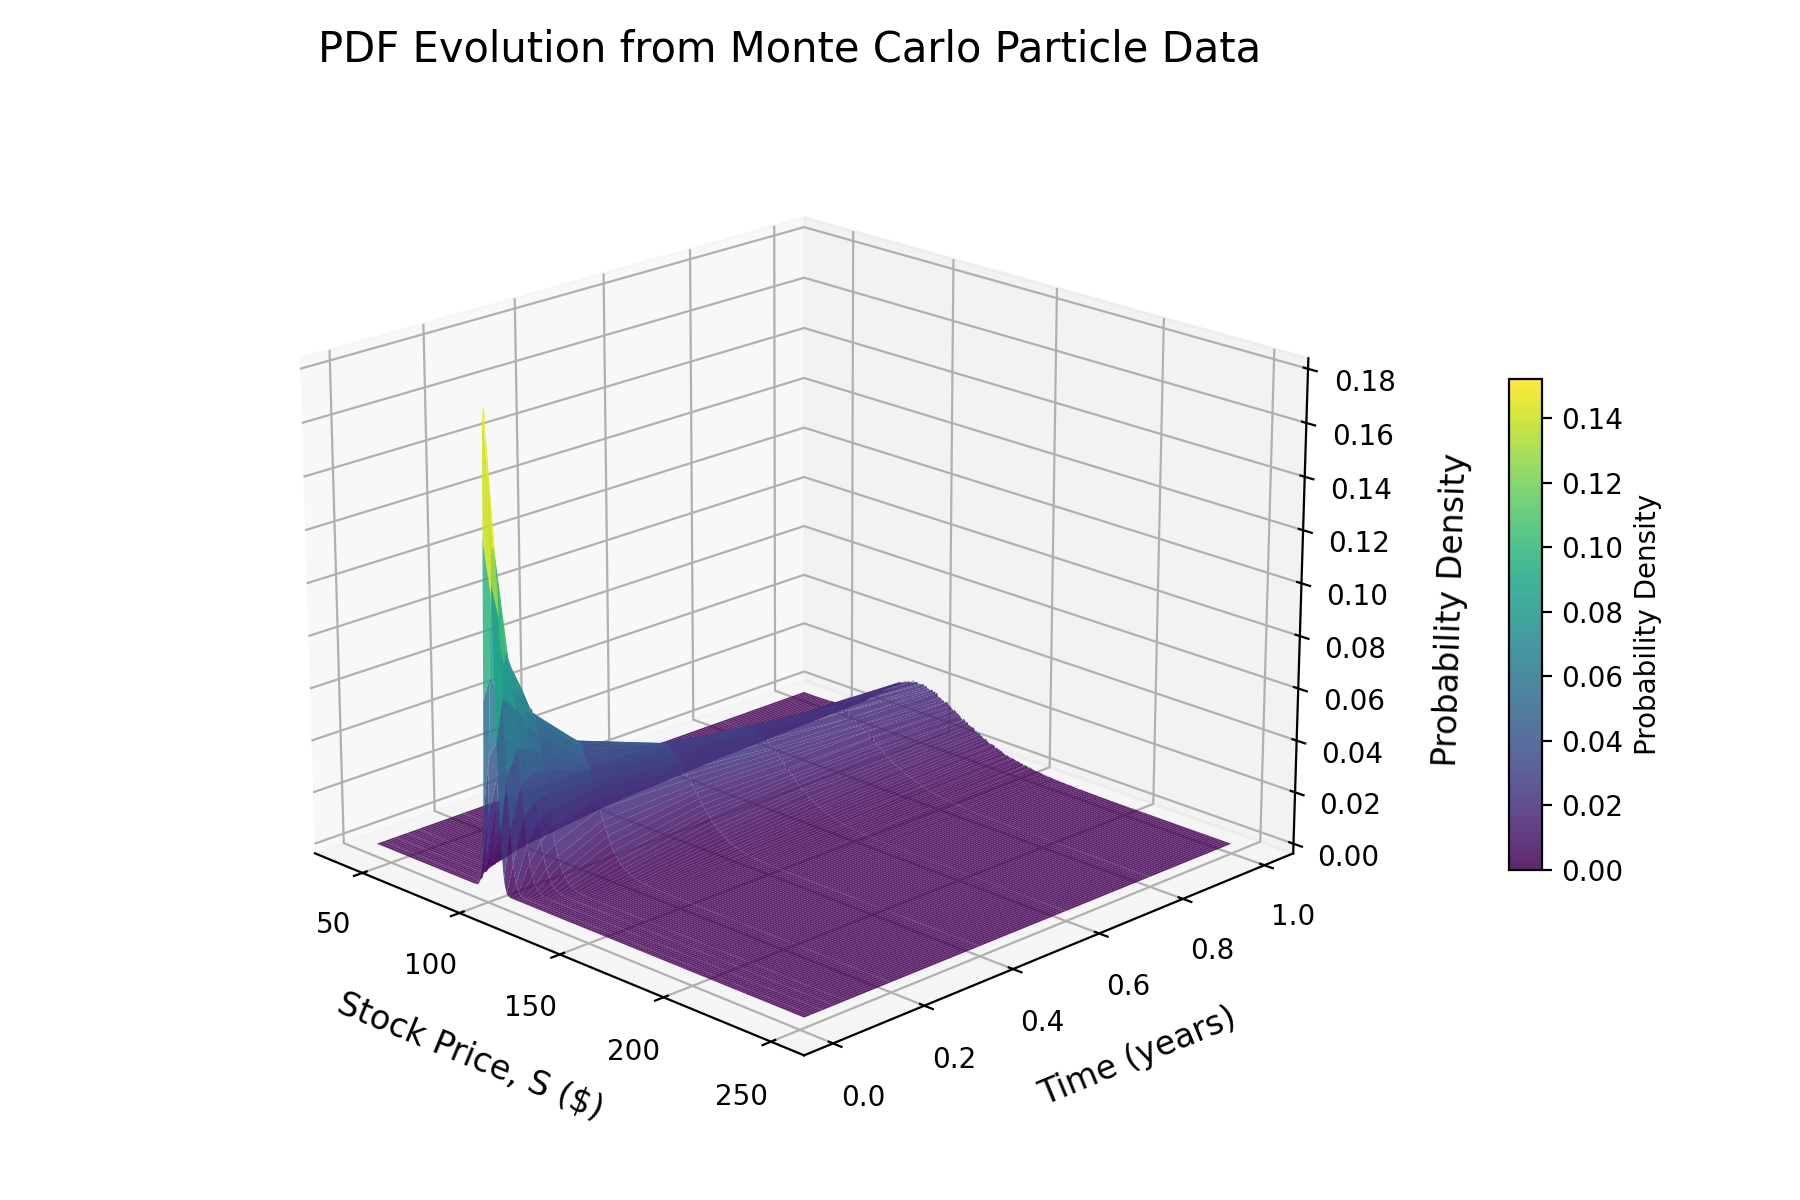
\includegraphics[width=\textwidth]{../BSM_Solver/figures/figure03_3d_pdf_evolution.png}
        \caption{PDF evolution from Monte Carlo particle data}
        \label{fig:residuals}
    \end{minipage}
\end{figure}

\subsection{Results: PDF Transport Continued}

TBD

\subsection{Results: Monte Carlo Convergence}

TBD

% ----------------------------------------------------------------------
% SECTION 08: CONCLUSIONS
% ----------------------------------------------------------------------
\section{Conclusions}

TBD


% ----------------------------------------------------------------------
% REFERENCES
% ----------------------------------------------------------------------
\nocite{*}
\newpage
\bibliographystyle{IEEEtran}
\bibliography{sources}

% ----------------------------------------------------------------------
% APPENDIX A: COPY OF PROGRAM LISTING
% ----------------------------------------------------------------------
\newpage
\appendix
\section{Copy of Program Listing}
\lstinputlisting[
    language=Python
]{../BSM_solver/bsm_solver.py}

\end{document}